\subsection{A matched training experiment limits the collapse claim}
All twelve new concentration arms complete 200 epochs, 3200 optimizer updates and 409600 cell presentations. Within each dataset--seed pair, the autoencoder initialization hash and saved batch/random schedule match; concentration-dependent prior buffers intentionally differ. No non-finite update is skipped and no run is selected by its score. Figure~\ref{fig:matched-training} and Table~\ref{tab:matched-training} retain all final states.

The fresh Setty comparison reproduces strict low-concentration collapse on two seeds, not all three. At $\alpha=0.1$, seeds 1 and 2 have maximum coordinate ranges $5.72\times10^{-13}$ and $1.74\times10^{-12}$, respectively; seed 0 has range 0.192837 and therefore fails the prespecified collapse criterion despite mean perplexity 1.002292. All three $\alpha=1$ Setty allocations are nondegenerate. Dentate has no strictly collapsed run at either concentration. In particular, Dentate seed 2 at $\alpha=0.1$ has mean perplexity approximately one but coordinate range one: different cells can occupy different corners. This observation directly demonstrates why within-cell concentration cannot stand in for between-cell collapse. The unfavorable replication for a universal-collapse claim is retained.
\begin{figure}[htbp]
\centering
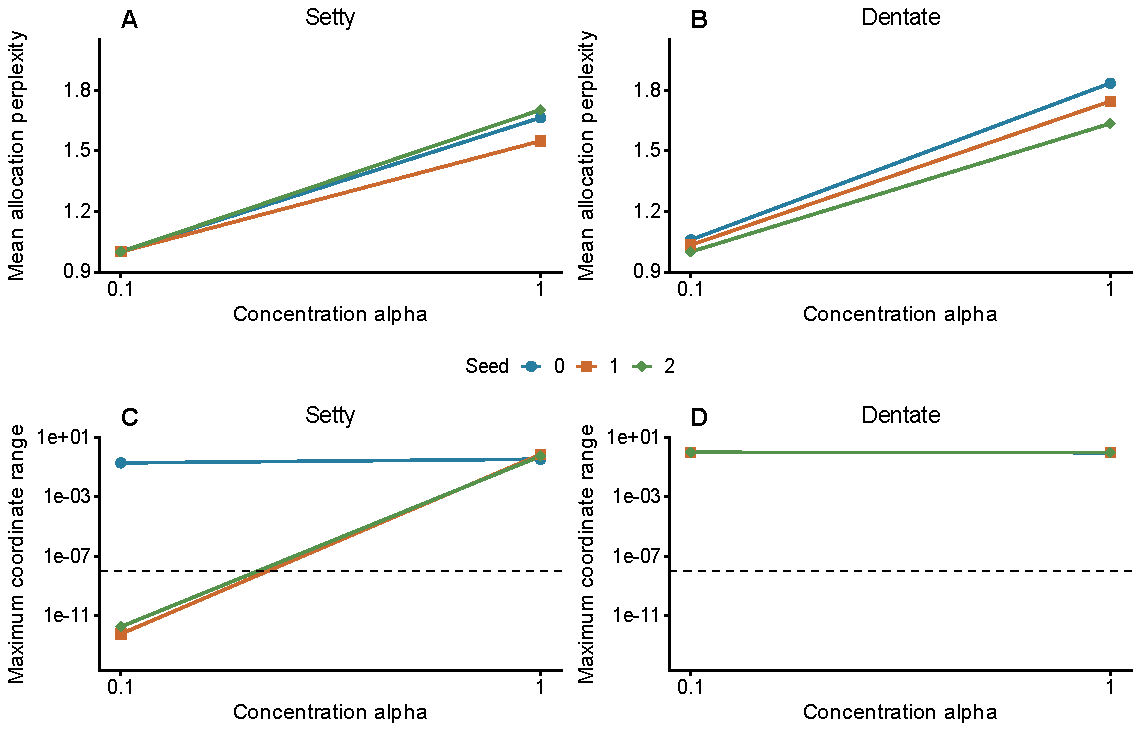
\includegraphics[width=.98\textwidth,height=0.72\textheight,keepaspectratio]{figures/matched_training.pdf}
\caption{\textbf{Matched concentration training.} A/B: Setty/Dentate mean perplexity. C/D: their maximum across-cell coordinate ranges on log scales. Lines join matched $\alpha=0.1$ and 1 endpoints; the inter-row key identifies seeds. Each point summarizes 450 cells, without seed averaging or error bars. All twelve arms complete 3200 updates and 409600 presentations. Strict collapse requires the dashed $10^{-8}$ range threshold and one occupied argmax topic. Perplexity near one alone is insufficient.}
\label{fig:matched-training}
\end{figure}
\begin{table}[htbp]
\centering
\caption{\textbf{All matched-training endpoints.} Range is the maximum over topic coordinates of the across-cell range. Occupancy counts distinct argmax topics. Strict collapse requires range at most $10^{-8}$ and occupancy one. The exact mean distinct-pair Jensen--Shannon divergence determines the separate degeneracy flag. Seed repetitions remain nested in two public data objects.}
\label{tab:matched-training}
\small
\begin{tabular}{llrrrrl}
\toprule
Dataset & Seed / $\alpha$ & Perplexity & Range & Occupancy & Pair JS & Collapse \\
\midrule
Setty & 0 / 0.1 & 1.0023 & 1.93e-01 & 1 & 4.87e-04 & no \\
Setty & 0 / 1 & 1.6640 & 3.45e-01 & 1 & 1.44e-02 & no \\
Setty & 1 / 0.1 & 1.0000 & 5.72e-13 & 1 & 2.39e-16 & yes \\
Setty & 1 / 1 & 1.5485 & 7.16e-01 & 2 & 4.78e-02 & no \\
Setty & 2 / 0.1 & 1.0000 & 1.74e-12 & 1 & 2.20e-15 & yes \\
Setty & 2 / 1 & 1.7029 & 5.54e-01 & 2 & 3.08e-02 & no \\
Dentate & 0 / 0.1 & 1.0591 & 1.00e+00 & 2 & 2.70e-01 & no \\
Dentate & 0 / 1 & 1.8347 & 9.40e-01 & 3 & 1.86e-01 & no \\
Dentate & 1 / 0.1 & 1.0334 & 1.00e+00 & 2 & 2.85e-01 & no \\
Dentate & 1 / 1 & 1.7450 & 9.61e-01 & 3 & 2.44e-01 & no \\
Dentate & 2 / 0.1 & 1.0000 & 1.00e+00 & 2 & 2.83e-01 & no \\
Dentate & 2 / 1 & 1.6351 & 9.65e-01 & 3 & 2.39e-01 & no \\
\bottomrule
\end{tabular}

\end{table}

Independent native-array recomputation confirms Setty $\alpha=0.1$: $2/3$ strict collapse (exact 95\% interval 0.094--0.992); Setty $\alpha=1$ and Dentate at both concentrations: each $0/3$ (0--0.708). All twelve classifications remain unchanged at exploratory range thresholds $10^{-10}$ and $10^{-6}$. Removing Setty seed 0 gives $2/2$ collapsed low-concentration runs, whereas removing seed 1 or 2 gives $1/2$; these are influence checks, not new replications. The seed-0 counterexample therefore remains consequential despite threshold stability. These intervals condition on fixed public objects and do not estimate donor or cohort prevalence. All 144 saved probe summaries also reproduce from their archived allocation arrays within float32 reduction tolerance.

\subsection{Trained-state implementation checks: token sensitivity and batch invariance}
The expected complete-token permutation and batch-context invariances check the implemented within-cell pathway; they are not scientific discoveries or evidence of attention as the cause of collapse.
Figure~\ref{fig:token-probes} tests every trained endpoint under both evaluation and zero-dropout training modes. Reversing complete tokens changes allocations by at most $4.77\times10^{-7}$, below the frozen $10^{-5}$ invariance tolerance. Altering the 48 companion cells or reversing batch order leaves the focal-cell allocations unchanged; isolated-cell evaluation differs by at most $9.84\times10^{-7}$. Thus these probes do not detect cross-cell mixing in the implemented deterministic encoder.

Content-changing interventions have a different response. Replacing all tokens by their per-cell mean gives an overall mean allocation $L_1$ change of 0.074070, while duplicating the first complete token gives 0.148893; individual coordinate changes can reach one. These averages combine the twelve endpoint states and two execution modes solely to describe probe magnitude, not independent biological replication. The per-state plot retains the heterogeneous responses. The result establishes sensitivity to token content in parts of the trained system, while providing no unique explanation of why two particular low-concentration runs collapsed.
\begin{figure}[htbp]
\centering
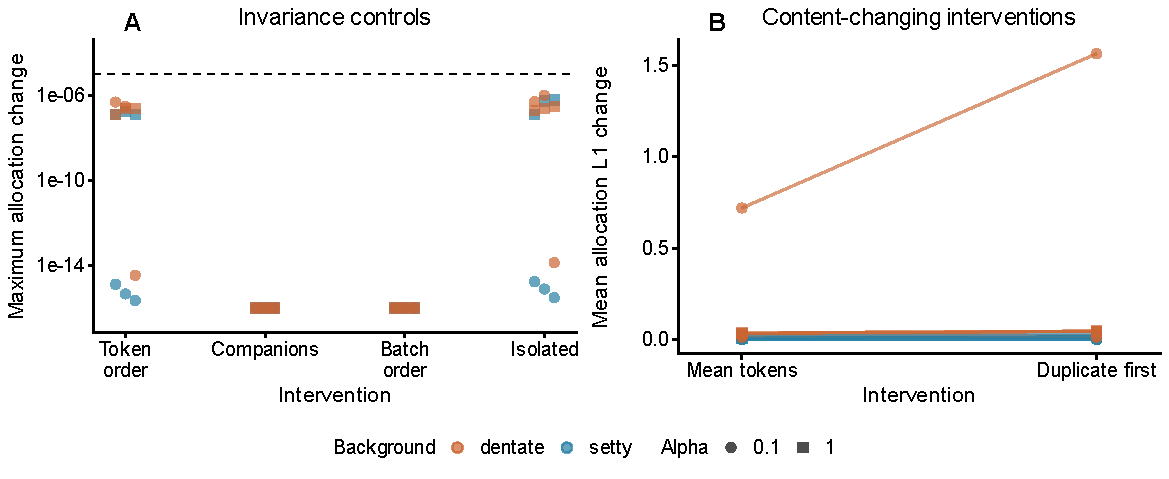
\includegraphics[width=.98\textwidth,height=0.72\textheight,keepaspectratio]{figures/token_probes.pdf}
\caption{\textbf{Trained-state token interventions.} A: maximum allocation change for token reversal, altered companions, restored batch reversal and isolated evaluation (log scale; values below $10^{-16}$ displayed at that floor). The dashed line marks the frozen $10^{-5}$ tolerance. B: mean row $L_1$ change under mean-token replacement and first-token duplication; lines join each state. Color/shape identify background/concentration. All twelve evaluation-mode states are retained without seed averaging or error bars. Probes use 64 test cells and 16 focal cells for context controls, with zero updates; training-mode probes use zero dropout.}
\label{fig:token-probes}
\end{figure}
